\documentclass[11pt, a4paper]{article}
\usepackage[a4paper, margin=1in]{geometry}

\usepackage{adjustbox}
\usepackage{mathtools}
\usepackage{amsmath}
\usepackage{amssymb}
\usepackage{amsthm}

\usepackage{pgfplots}
\usepackage{listings}
\usepackage{color}
\usepackage{tikz}

\usepackage{textcomp}
\usepackage{soul}

\usepackage[hidelinks]{hyperref}
\pgfplotsset{width=7.5cm,compat=1.12}
\usepgfplotslibrary{fillbetween}
\pgfplotsset{compat=1.8}
\usepgfplotslibrary{statistics}
\usepackage[makeroom]{cancel}
\title{\bf{Homework \textnumero 5}}
\author{Author: David Oniani
\\
\ \ \ Instructor: Dr. Eric Westlund}
\date{February 20, 2019}

\usepackage{listings}
\usepackage{color}

%%%%%%%%%%%%%%% S E T S %%%%%%%%%%%%%%%
\newcommand{\nats}{\mathbb{N}}
\newcommand{\ints}{\mathbb{Z}}
\newcommand{\rats}{\mathbb{Q}}
\newcommand{\reals}{\mathbb{R}}
\newcommand{\irrats}{\mathbb{I}}

\newcommand{\pnats}{\mathbb{N}^+}
\newcommand{\pints}{\mathbb{Z}^+}
\newcommand{\prats}{\mathbb{Q}^+}
\newcommand{\preals}{\mathbb{R}^+}
\newcommand{\nreals}{\mathbb{R}^-}

\newcommand{\nints}{\mathbb{Z}^-}
\newcommand{\nrats}{\mathbb{Q}^-}
%%%%%%%%%%%%%%%%%%%%%%%%%%%%%%%%%%%%%%%

% Calligraphy
\newcommand\und[1]{\underline{\smash{#1}}}

% Operators
\DeclarePairedDelimiter\abs{\lvert}{\rvert}
\DeclarePairedDelimiter\ceil{\lceil}{\rceil}
\DeclarePairedDelimiter\floor{\lfloor}{\rfloor}

% Other
\newcommand{\rarr}{\rightarrow}

\definecolor{dkgreen}{rgb}{0,0.6,0}
\definecolor{gray}{rgb}{0.5,0.5,0.5}
\definecolor{mauve}{rgb}{0.58,0,0.82}
\definecolor{backcolour}{rgb}{0.95,0.95,0.92}

\lstset{
backgroundcolor=\color{backcolour},
aboveskip=3mm,
belowskip=3mm,
showstringspaces=false,
columns=flexible,
basicstyle={\small\ttfamily},
numbers=left,
numberstyle=\normalsize\color{gray},
keywordstyle=\color{blue},
commentstyle=\color{dkgreen},
stringstyle=\color{mauve},
breaklines=true,
breakatwhitespace=true,
tabsize=4
}


\begin{document}
\maketitle
\begin{itemize}
\item[5.1]
\begin{itemize}
\item[(a)]
The slope is 1.033. Slope is the rate of change. Particularly,
it tells us that highway mileage increases by 1.016 for every
1 mpg change in the city mileage.

\item[]

\item[(b)]
The intercept is 6.785. This would be a mileage for a car
with 0 mpg and such car would probably not be present.

\item[]

\item[(c)]
Let's plug the numbers. For $\text{city mpg} = 16$, we get $\text{highway mpg} = 6.785 + (1.033 \times 16) = 23.313$. And for $\text{city mpg} = 28$, we get $\text{highway mpg} = 6.785 + (1.033 \times 28) = 35.709$.

\item[]

\item[(d)]
\item[]
\item[]
\begin{center}
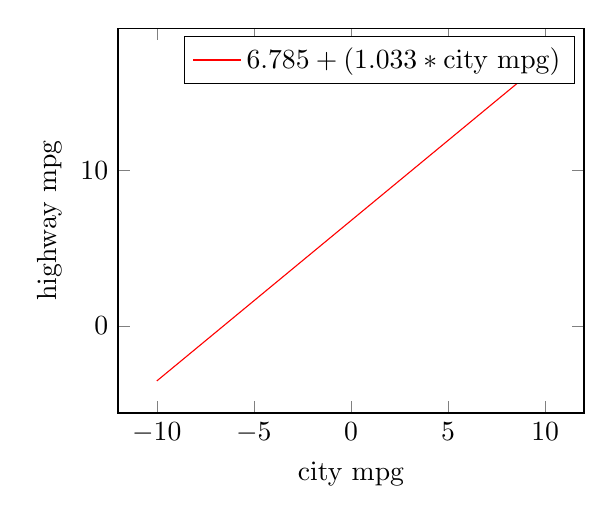
\begin{tikzpicture}
\begin{axis}[
    xlabel = $\text{city mpg}$,
    ylabel = $\text{highway mpg}$,
]

\addplot [
    domain=-10:10,
    samples=1000, 
    color=red,
]
{6.785 + (1.033 * x)};
\addlegendentry{$6.785 + (1.033 * \text{city mpg})$}
\end{axis}
\end{tikzpicture}
\end{center}
\item[]
\item[]
\end{itemize}

\newpage

\item[5.5]
\begin{itemize}
\item[(a)]
Below is the scatterplot for the data.

\item[]
\item[]
\begin{center}
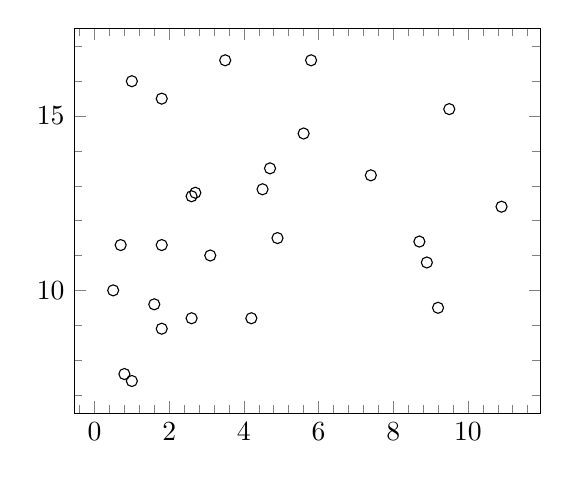
\begin{tikzpicture}
\begin{axis}[%
scatter/classes={%
    a={mark=o,draw=black}},
    minor y tick num = 4,
    minor x tick num = 4]
\addplot[scatter,only marks,%
    scatter src=explicit symbolic]%
table[meta=label] {
x y label
4.2 9.2 a
1.8 15.5 a
2.6 12.7 a
1.0 16.0 a
5.6 14.5 a
3.5 16.6 a
9.2 9.5 a
0.8 7.6 a
8.7 11.4 a
2.7 12.8 a
8.9 10.8 a
1.8 11.3 a
4.5 12.9 a
3.1 11.0 a
7.4 13.3 a
10.9 12.4 a
0.5 10.0 a
2.6 9.2 a
9.5 15.2 a
1.6 9.6 a
4.7 13.5 a
4.9 11.5 a
5.8 16.6 a
0.7 11.3 a
1.8 8.9 a
1.0 7.4 a
    };
\end{axis}
\end{tikzpicture}
\end{center}
\item[]

\item[(b)]
Using the \texttt{Haskell} library \texttt{Statistics.LinearRegression} (link: \url{https://bit.ly/2BLQ7Qb}), we get the regression line $y = 11.125 + 0.195x$. Below is the plot with the line added.
\item[]
\item[]
\begin{center}
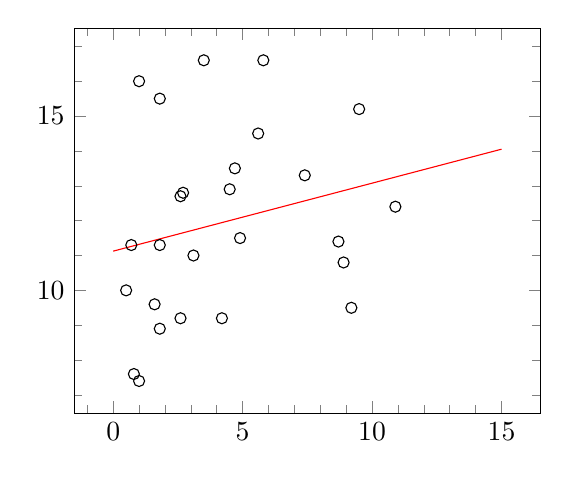
\begin{tikzpicture}
\begin{axis}[%
domain = 0:15,
scatter/classes={%
    a={mark=o,draw=black}},
    minor y tick num = 4,
    minor x tick num = 4]
\addplot[scatter,only marks,%
    scatter src=explicit symbolic]%
table[meta=label] {
x y label
4.2 9.2 a
1.8 15.5 a
2.6 12.7 a
1.0 16.0 a
5.6 14.5 a
3.5 16.6 a
9.2 9.5 a
0.8 7.6 a
8.7 11.4 a
2.7 12.8 a
8.9 10.8 a
1.8 11.3 a
4.5 12.9 a
3.1 11.0 a
7.4 13.3 a
10.9 12.4 a
0.5 10.0 a
2.6 9.2 a
9.5 15.2 a
1.6 9.6 a
4.7 13.5 a
4.9 11.5 a
5.8 16.6 a
0.7 11.3 a
1.8 8.9 a
1.0 7.4 a
    };

\textbf{\addplot [
    samples=1000,
    color=red,
]
{11.125 + 0.195 * x};}
\end{axis}

\end{tikzpicture}
\end{center}


\item[]

\item[(c)]
It tells us the expected increase. Particularly, it tells
us that for every suicide, there are approximately 0.195 homicides.

\item[]

\item[(d)]
We can just plug the value in the regression equation.
We get: $\hat{y} = 11.125 + 0.195 \times 8.0 = 12.685$.
Therefore, the rate is 12.685 per 100, 000 people.
\end{itemize}

\newpage

\item[5.9]
\begin{itemize}
\item[(a)]
\item[]
\item[]
\begin{center}
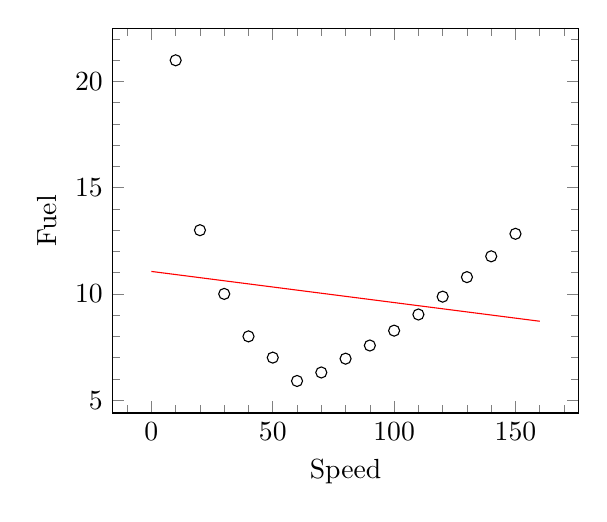
\begin{tikzpicture}
\begin{axis}[%
    domain = 0:160,
    xlabel = $\text{Speed}$,
    ylabel = $\text{Fuel}$,
    scatter/classes={a={mark=o,draw=black}},
    minor y tick num = 4,
    minor x tick num = 4]
\addplot[scatter,only marks,%
    scatter src=explicit symbolic]%
table[meta=label] {
x y label
10 21.00 a
20 13.00 a
30 10.00 a
40 8.00 a
50 7.00 a
60 5.90 a
70 6.30 a
80 6.95 a
90 7.57 a
100 8.27 a
110 9.03 a
120 9.87 a
130 10.79 a
140 11.77 a
150 12.83 a
    };

\textbf{\addplot [
    samples=1000,
    color=red,
]
{11.058 - 0.01466 * x};}
\end{axis}
\end{tikzpicture}
\end{center}

\item[]

\item[(b)]
It is clear that the relationship between the speed and fuel
is parabolic. Therefore, predictions based on the output of
the give regression line would be inaccurate. Hence,
the answer is NO.

\item[]

\item[(c)]
We have: $11.058 - 0.01466 \times 10 = 10.9114$.
Then, we know that the residual is predicted
value minus the actual value which gives us $21 - 10.9114 = 10.0886$.
After rounding $10.0886$, we indeed get $10.09$ which is the
residual value on the table.
\end{itemize}

\item[]


\item[(d)]
\item[]
\item[]
\begin{center}
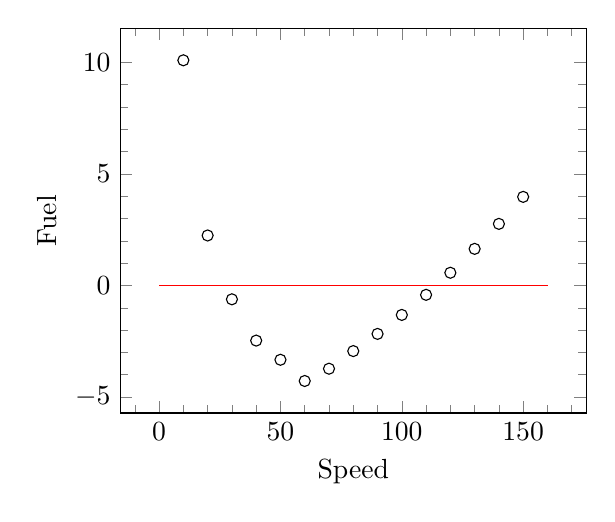
\begin{tikzpicture}
\begin{axis}[%
    domain = 0:160,
    xlabel = $\text{Speed}$,
    ylabel = $\text{Fuel}$,
    scatter/classes={a={mark=o,draw=black}},
    minor y tick num = 4,
    minor x tick num = 4]
\addplot[scatter,only marks,%
    scatter src=explicit symbolic]%
table[meta=label] {
x y label
10 10.09 a
20 2.24 a
30 -0.62 a
40 -2.47 a
50 -3.33 a
60 -4.28 a
70 -3.73 a
80 -2.94 a
90 -2.17 a
100 -1.32 a
110 -0.42 a
120 0.57 a
130 1.64 a
140 2.76 a
150 3.97 a
    };

\textbf{\addplot [
    samples=1000,
    color=red,
]
{0};}
\end{axis}
\end{tikzpicture}
\end{center}
The pattern seems to be virtually the same as the pattern
exhibited in the part (a) of this exercise.
\item[]
\item[]

\newpage

\item[5.15]
\begin{itemize}
\item[(a)]
Once again, using the software, we get that the regression
line is $\hat{y} = -44.831 + 0.132x$.

\item[]

\item[(b)]
The prediction would be $-44.831 + 0.132 \times 890 \approx 73$.
We can trust this prediction since 890 is in-between (but not outside)
the table values (observed values).

\item[]

\item[(c)]
That happens if $x = 0$. In this case we get that
-44.831 manatees are killed which does not seem reasonable.
This happens since 0 is outside the range of table values.
\end{itemize}

\item[]
\item[]

\item[5.17]
Income, parents' (or mother's) IQ. There might also be some other
genetic reasons which did not show up in mother but did in her
child(ren).

\item[]
\item[]

\item[5.34]
\begin{itemize}
\item[(a)]
The slope is $m = r \times \dfrac{s_y}{s_x} = 0.5 \times \dfrac{3.1}{2.7} \approx 0.59$.\\
The intercept is $b = \bar{y} - m \times \bar{x} = 69.9 - 0.59 \times 64.3 = 31.96$.
\item[]

\item[(b)]
The regression line equation is $\hat{y} = 31.96 + 0.59x$.
For $x = 67$, we get $\approx 71.5$.
\item[]
\item[]
\begin{center}
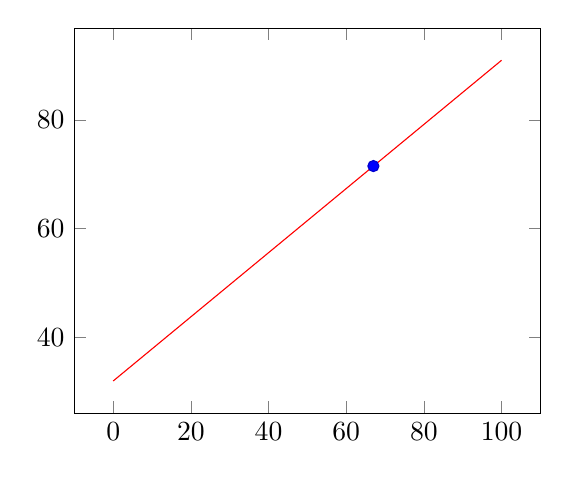
\begin{tikzpicture}
\begin{axis}[domain=0:100]
\addplot[scatter,only marks]%
table[meta=label] {
x y label
67 71.5 a
    };
\addplot [
    samples=1000,
    color=red,
]
{31.96 + 0.59 * x};
\end{axis}
\end{tikzpicture}
\end{center}
\item[]
\item[]

\item[]

\item[(c)]
The regression line only explains $r^2$ which is $25\%$ of the variation in the height of the husband.
\end{itemize}

\item[]
\item[]

\item[5.35]
\begin{itemize}
\item[(a)]
The slope is $m = 0.5 \times \dfrac{8}{40} = 0.1$.\\
The intercept is $b = 75 - 0.1 \times 280 = 47$.\\
The regression line equation is $\hat{y} = 47 + 0.1x$

\item[]

\item[(b)]
We just plug in the value 300 and get $47 + 0.1 \times 300 = 77$.

\item[]

\item[(c)]
I actually agree with Julie. The regression line explains only
$r^2$ which is $25\%$ variation in student final exam scores.
\end{itemize}

\item[]
\item[]

\item[5.55]
Predicted second-round score for a player who shot 80 is $56.47 + 0.243 \times 80 = 75.91$.\\
Predicted second-round score for a player who shot 70 is $56.47 + 0.243 \times 70 = 73.48$.\\\\
The player who shot 80 in the first round is predicted to score below
the average, but overall, a better score.\\
The player who shot 80 in the first round is predicted to score above
the average, but overall, a worse score.

\item[]
\item[]

\item[5.56]
We know that the point $(\overline{x}, \overline{y})$ lies
on the least squares regression line. Then equality $\overline{y} = 46.6 + 0.41\overline{x}$ holds. Since Octavio scored $\overline{x}$ 10 points
above the mean, it means that he scored $\overline{x} + 10$. We can
now plug this value in the regression equation to get $\hat{y} = 46.6 + 0.41 \times (\overline{x} + 10) = 46.6 + 0,41\overline{x} + 4.1 = \overline{y} + 4.1$. Finally, we got that $\hat{y} = \overline{y} + 4.1$
which means that Octavio's final exam score is predicted to be 4.1 points
above the class mean on that final exam.
\end{itemize}
\end{document}
